
% Default to the notebook output style

    


% Inherit from the specified cell style.




    
\documentclass[11pt]{article}

    
    
    \usepackage[UTF8]{ctex} %This is what i added
    \usepackage[T1]{fontenc}
    % Nicer default font than Computer Modern for most use cases
    \usepackage{palatino}

    % Basic figure setup, for now with no caption control since it's done
    % automatically by Pandoc (which extracts ![](path) syntax from Markdown).
    \usepackage{graphicx}
    % We will generate all images so they have a width \maxwidth. This means
    % that they will get their normal width if they fit onto the page, but
    % are scaled down if they would overflow the margins.
    \makeatletter
    \def\maxwidth{\ifdim\Gin@nat@width>\linewidth\linewidth
    \else\Gin@nat@width\fi}
    \makeatother
    \let\Oldincludegraphics\includegraphics
    % Set max figure width to be 80% of text width, for now hardcoded.
    \renewcommand{\includegraphics}[1]{\Oldincludegraphics[width=.8\maxwidth]{#1}}
    % Ensure that by default, figures have no caption (until we provide a
    % proper Figure object with a Caption API and a way to capture that
    % in the conversion process - todo).
    \usepackage{caption}
    \DeclareCaptionLabelFormat{nolabel}{}
    \captionsetup{labelformat=nolabel}

    \usepackage{adjustbox} % Used to constrain images to a maximum size 
    \usepackage{xcolor} % Allow colors to be defined
    \usepackage{enumerate} % Needed for markdown enumerations to work
    \usepackage{geometry} % Used to adjust the document margins
    \usepackage{amsmath} % Equations
    \usepackage{amssymb} % Equations
    \usepackage{textcomp} % defines textquotesingle
    % Hack from http://tex.stackexchange.com/a/47451/13684:
    \AtBeginDocument{%
        \def\PYZsq{\textquotesingle}% Upright quotes in Pygmentized code
    }
    \usepackage{upquote} % Upright quotes for verbatim code
    \usepackage{eurosym} % defines \euro
    \usepackage[mathletters]{ucs} % Extended unicode (utf-8) support
    %\usepackage[utf8x]{inputenc} % Allow utf-8 characters in the tex document
    \usepackage{fancyvrb} % verbatim replacement that allows latex
    \usepackage{grffile} % extends the file name processing of package graphics 
                         % to support a larger range 
    % The hyperref package gives us a pdf with properly built
    % internal navigation ('pdf bookmarks' for the table of contents,
    % internal cross-reference links, web links for URLs, etc.)
    \usepackage{hyperref}
    \usepackage{longtable} % longtable support required by pandoc >1.10
    \usepackage{booktabs}  % table support for pandoc > 1.12.2
    %\usepackage[normalem]{ulem} % ulem is needed to support strikethroughs (\sout)
                                % normalem makes italics be italics, not underlines
    

    
    
    % Colors for the hyperref package
    \definecolor{urlcolor}{rgb}{0,.145,.698}
    \definecolor{linkcolor}{rgb}{.71,0.21,0.01}
    \definecolor{citecolor}{rgb}{.12,.54,.11}

    % ANSI colors
    \definecolor{ansi-black}{HTML}{3E424D}
    \definecolor{ansi-black-intense}{HTML}{282C36}
    \definecolor{ansi-red}{HTML}{E75C58}
    \definecolor{ansi-red-intense}{HTML}{B22B31}
    \definecolor{ansi-green}{HTML}{00A250}
    \definecolor{ansi-green-intense}{HTML}{007427}
    \definecolor{ansi-yellow}{HTML}{DDB62B}
    \definecolor{ansi-yellow-intense}{HTML}{B27D12}
    \definecolor{ansi-blue}{HTML}{208FFB}
    \definecolor{ansi-blue-intense}{HTML}{0065CA}
    \definecolor{ansi-magenta}{HTML}{D160C4}
    \definecolor{ansi-magenta-intense}{HTML}{A03196}
    \definecolor{ansi-cyan}{HTML}{60C6C8}
    \definecolor{ansi-cyan-intense}{HTML}{258F8F}
    \definecolor{ansi-white}{HTML}{C5C1B4}
    \definecolor{ansi-white-intense}{HTML}{A1A6B2}

    % commands and environments needed by pandoc snippets
    % extracted from the output of `pandoc -s`
    \providecommand{\tightlist}{%
      \setlength{\itemsep}{0pt}\setlength{\parskip}{0pt}}
    \DefineVerbatimEnvironment{Highlighting}{Verbatim}{commandchars=\\\{\}}
    % Add ',fontsize=\small' for more characters per line
    \newenvironment{Shaded}{}{}
    \newcommand{\KeywordTok}[1]{\textcolor[rgb]{0.00,0.44,0.13}{\textbf{{#1}}}}
    \newcommand{\DataTypeTok}[1]{\textcolor[rgb]{0.56,0.13,0.00}{{#1}}}
    \newcommand{\DecValTok}[1]{\textcolor[rgb]{0.25,0.63,0.44}{{#1}}}
    \newcommand{\BaseNTok}[1]{\textcolor[rgb]{0.25,0.63,0.44}{{#1}}}
    \newcommand{\FloatTok}[1]{\textcolor[rgb]{0.25,0.63,0.44}{{#1}}}
    \newcommand{\CharTok}[1]{\textcolor[rgb]{0.25,0.44,0.63}{{#1}}}
    \newcommand{\StringTok}[1]{\textcolor[rgb]{0.25,0.44,0.63}{{#1}}}
    \newcommand{\CommentTok}[1]{\textcolor[rgb]{0.38,0.63,0.69}{\textit{{#1}}}}
    \newcommand{\OtherTok}[1]{\textcolor[rgb]{0.00,0.44,0.13}{{#1}}}
    \newcommand{\AlertTok}[1]{\textcolor[rgb]{1.00,0.00,0.00}{\textbf{{#1}}}}
    \newcommand{\FunctionTok}[1]{\textcolor[rgb]{0.02,0.16,0.49}{{#1}}}
    \newcommand{\RegionMarkerTok}[1]{{#1}}
    \newcommand{\ErrorTok}[1]{\textcolor[rgb]{1.00,0.00,0.00}{\textbf{{#1}}}}
    \newcommand{\NormalTok}[1]{{#1}}
    
    % Additional commands for more recent versions of Pandoc
    \newcommand{\ConstantTok}[1]{\textcolor[rgb]{0.53,0.00,0.00}{{#1}}}
    \newcommand{\SpecialCharTok}[1]{\textcolor[rgb]{0.25,0.44,0.63}{{#1}}}
    \newcommand{\VerbatimStringTok}[1]{\textcolor[rgb]{0.25,0.44,0.63}{{#1}}}
    \newcommand{\SpecialStringTok}[1]{\textcolor[rgb]{0.73,0.40,0.53}{{#1}}}
    \newcommand{\ImportTok}[1]{{#1}}
    \newcommand{\DocumentationTok}[1]{\textcolor[rgb]{0.73,0.13,0.13}{\textit{{#1}}}}
    \newcommand{\AnnotationTok}[1]{\textcolor[rgb]{0.38,0.63,0.69}{\textbf{\textit{{#1}}}}}
    \newcommand{\CommentVarTok}[1]{\textcolor[rgb]{0.38,0.63,0.69}{\textbf{\textit{{#1}}}}}
    \newcommand{\VariableTok}[1]{\textcolor[rgb]{0.10,0.09,0.49}{{#1}}}
    \newcommand{\ControlFlowTok}[1]{\textcolor[rgb]{0.00,0.44,0.13}{\textbf{{#1}}}}
    \newcommand{\OperatorTok}[1]{\textcolor[rgb]{0.40,0.40,0.40}{{#1}}}
    \newcommand{\BuiltInTok}[1]{{#1}}
    \newcommand{\ExtensionTok}[1]{{#1}}
    \newcommand{\PreprocessorTok}[1]{\textcolor[rgb]{0.74,0.48,0.00}{{#1}}}
    \newcommand{\AttributeTok}[1]{\textcolor[rgb]{0.49,0.56,0.16}{{#1}}}
    \newcommand{\InformationTok}[1]{\textcolor[rgb]{0.38,0.63,0.69}{\textbf{\textit{{#1}}}}}
    \newcommand{\WarningTok}[1]{\textcolor[rgb]{0.38,0.63,0.69}{\textbf{\textit{{#1}}}}}
    
    
    % Define a nice break command that doesn't care if a line doesn't already
    % exist.
    \def\br{\hspace*{\fill} \\* }
    % Math Jax compatability definitions
    \def\gt{>}
    \def\lt{<}
    % Document parameters
    \title{评论|制度与文化如何影响个体行为}
    \author{王耀}
    
    
    

    % Pygments definitions
    
\makeatletter
\def\PY@reset{\let\PY@it=\relax \let\PY@bf=\relax%
    \let\PY@ul=\relax \let\PY@tc=\relax%
    \let\PY@bc=\relax \let\PY@ff=\relax}
\def\PY@tok#1{\csname PY@tok@#1\endcsname}
\def\PY@toks#1+{\ifx\relax#1\empty\else%
    \PY@tok{#1}\expandafter\PY@toks\fi}
\def\PY@do#1{\PY@bc{\PY@tc{\PY@ul{%
    \PY@it{\PY@bf{\PY@ff{#1}}}}}}}
\def\PY#1#2{\PY@reset\PY@toks#1+\relax+\PY@do{#2}}

\expandafter\def\csname PY@tok@gd\endcsname{\def\PY@tc##1{\textcolor[rgb]{0.63,0.00,0.00}{##1}}}
\expandafter\def\csname PY@tok@gu\endcsname{\let\PY@bf=\textbf\def\PY@tc##1{\textcolor[rgb]{0.50,0.00,0.50}{##1}}}
\expandafter\def\csname PY@tok@gt\endcsname{\def\PY@tc##1{\textcolor[rgb]{0.00,0.27,0.87}{##1}}}
\expandafter\def\csname PY@tok@gs\endcsname{\let\PY@bf=\textbf}
\expandafter\def\csname PY@tok@gr\endcsname{\def\PY@tc##1{\textcolor[rgb]{1.00,0.00,0.00}{##1}}}
\expandafter\def\csname PY@tok@cm\endcsname{\let\PY@it=\textit\def\PY@tc##1{\textcolor[rgb]{0.25,0.50,0.50}{##1}}}
\expandafter\def\csname PY@tok@vg\endcsname{\def\PY@tc##1{\textcolor[rgb]{0.10,0.09,0.49}{##1}}}
\expandafter\def\csname PY@tok@vi\endcsname{\def\PY@tc##1{\textcolor[rgb]{0.10,0.09,0.49}{##1}}}
\expandafter\def\csname PY@tok@mh\endcsname{\def\PY@tc##1{\textcolor[rgb]{0.40,0.40,0.40}{##1}}}
\expandafter\def\csname PY@tok@cs\endcsname{\let\PY@it=\textit\def\PY@tc##1{\textcolor[rgb]{0.25,0.50,0.50}{##1}}}
\expandafter\def\csname PY@tok@ge\endcsname{\let\PY@it=\textit}
\expandafter\def\csname PY@tok@vc\endcsname{\def\PY@tc##1{\textcolor[rgb]{0.10,0.09,0.49}{##1}}}
\expandafter\def\csname PY@tok@il\endcsname{\def\PY@tc##1{\textcolor[rgb]{0.40,0.40,0.40}{##1}}}
\expandafter\def\csname PY@tok@go\endcsname{\def\PY@tc##1{\textcolor[rgb]{0.53,0.53,0.53}{##1}}}
\expandafter\def\csname PY@tok@cp\endcsname{\def\PY@tc##1{\textcolor[rgb]{0.74,0.48,0.00}{##1}}}
\expandafter\def\csname PY@tok@gi\endcsname{\def\PY@tc##1{\textcolor[rgb]{0.00,0.63,0.00}{##1}}}
\expandafter\def\csname PY@tok@gh\endcsname{\let\PY@bf=\textbf\def\PY@tc##1{\textcolor[rgb]{0.00,0.00,0.50}{##1}}}
\expandafter\def\csname PY@tok@ni\endcsname{\let\PY@bf=\textbf\def\PY@tc##1{\textcolor[rgb]{0.60,0.60,0.60}{##1}}}
\expandafter\def\csname PY@tok@nl\endcsname{\def\PY@tc##1{\textcolor[rgb]{0.63,0.63,0.00}{##1}}}
\expandafter\def\csname PY@tok@nn\endcsname{\let\PY@bf=\textbf\def\PY@tc##1{\textcolor[rgb]{0.00,0.00,1.00}{##1}}}
\expandafter\def\csname PY@tok@no\endcsname{\def\PY@tc##1{\textcolor[rgb]{0.53,0.00,0.00}{##1}}}
\expandafter\def\csname PY@tok@na\endcsname{\def\PY@tc##1{\textcolor[rgb]{0.49,0.56,0.16}{##1}}}
\expandafter\def\csname PY@tok@nb\endcsname{\def\PY@tc##1{\textcolor[rgb]{0.00,0.50,0.00}{##1}}}
\expandafter\def\csname PY@tok@nc\endcsname{\let\PY@bf=\textbf\def\PY@tc##1{\textcolor[rgb]{0.00,0.00,1.00}{##1}}}
\expandafter\def\csname PY@tok@nd\endcsname{\def\PY@tc##1{\textcolor[rgb]{0.67,0.13,1.00}{##1}}}
\expandafter\def\csname PY@tok@ne\endcsname{\let\PY@bf=\textbf\def\PY@tc##1{\textcolor[rgb]{0.82,0.25,0.23}{##1}}}
\expandafter\def\csname PY@tok@nf\endcsname{\def\PY@tc##1{\textcolor[rgb]{0.00,0.00,1.00}{##1}}}
\expandafter\def\csname PY@tok@si\endcsname{\let\PY@bf=\textbf\def\PY@tc##1{\textcolor[rgb]{0.73,0.40,0.53}{##1}}}
\expandafter\def\csname PY@tok@s2\endcsname{\def\PY@tc##1{\textcolor[rgb]{0.73,0.13,0.13}{##1}}}
\expandafter\def\csname PY@tok@nt\endcsname{\let\PY@bf=\textbf\def\PY@tc##1{\textcolor[rgb]{0.00,0.50,0.00}{##1}}}
\expandafter\def\csname PY@tok@nv\endcsname{\def\PY@tc##1{\textcolor[rgb]{0.10,0.09,0.49}{##1}}}
\expandafter\def\csname PY@tok@s1\endcsname{\def\PY@tc##1{\textcolor[rgb]{0.73,0.13,0.13}{##1}}}
\expandafter\def\csname PY@tok@ch\endcsname{\let\PY@it=\textit\def\PY@tc##1{\textcolor[rgb]{0.25,0.50,0.50}{##1}}}
\expandafter\def\csname PY@tok@m\endcsname{\def\PY@tc##1{\textcolor[rgb]{0.40,0.40,0.40}{##1}}}
\expandafter\def\csname PY@tok@gp\endcsname{\let\PY@bf=\textbf\def\PY@tc##1{\textcolor[rgb]{0.00,0.00,0.50}{##1}}}
\expandafter\def\csname PY@tok@sh\endcsname{\def\PY@tc##1{\textcolor[rgb]{0.73,0.13,0.13}{##1}}}
\expandafter\def\csname PY@tok@ow\endcsname{\let\PY@bf=\textbf\def\PY@tc##1{\textcolor[rgb]{0.67,0.13,1.00}{##1}}}
\expandafter\def\csname PY@tok@sx\endcsname{\def\PY@tc##1{\textcolor[rgb]{0.00,0.50,0.00}{##1}}}
\expandafter\def\csname PY@tok@bp\endcsname{\def\PY@tc##1{\textcolor[rgb]{0.00,0.50,0.00}{##1}}}
\expandafter\def\csname PY@tok@c1\endcsname{\let\PY@it=\textit\def\PY@tc##1{\textcolor[rgb]{0.25,0.50,0.50}{##1}}}
\expandafter\def\csname PY@tok@o\endcsname{\def\PY@tc##1{\textcolor[rgb]{0.40,0.40,0.40}{##1}}}
\expandafter\def\csname PY@tok@kc\endcsname{\let\PY@bf=\textbf\def\PY@tc##1{\textcolor[rgb]{0.00,0.50,0.00}{##1}}}
\expandafter\def\csname PY@tok@c\endcsname{\let\PY@it=\textit\def\PY@tc##1{\textcolor[rgb]{0.25,0.50,0.50}{##1}}}
\expandafter\def\csname PY@tok@mf\endcsname{\def\PY@tc##1{\textcolor[rgb]{0.40,0.40,0.40}{##1}}}
\expandafter\def\csname PY@tok@err\endcsname{\def\PY@bc##1{\setlength{\fboxsep}{0pt}\fcolorbox[rgb]{1.00,0.00,0.00}{1,1,1}{\strut ##1}}}
\expandafter\def\csname PY@tok@mb\endcsname{\def\PY@tc##1{\textcolor[rgb]{0.40,0.40,0.40}{##1}}}
\expandafter\def\csname PY@tok@ss\endcsname{\def\PY@tc##1{\textcolor[rgb]{0.10,0.09,0.49}{##1}}}
\expandafter\def\csname PY@tok@sr\endcsname{\def\PY@tc##1{\textcolor[rgb]{0.73,0.40,0.53}{##1}}}
\expandafter\def\csname PY@tok@mo\endcsname{\def\PY@tc##1{\textcolor[rgb]{0.40,0.40,0.40}{##1}}}
\expandafter\def\csname PY@tok@kd\endcsname{\let\PY@bf=\textbf\def\PY@tc##1{\textcolor[rgb]{0.00,0.50,0.00}{##1}}}
\expandafter\def\csname PY@tok@mi\endcsname{\def\PY@tc##1{\textcolor[rgb]{0.40,0.40,0.40}{##1}}}
\expandafter\def\csname PY@tok@kn\endcsname{\let\PY@bf=\textbf\def\PY@tc##1{\textcolor[rgb]{0.00,0.50,0.00}{##1}}}
\expandafter\def\csname PY@tok@cpf\endcsname{\let\PY@it=\textit\def\PY@tc##1{\textcolor[rgb]{0.25,0.50,0.50}{##1}}}
\expandafter\def\csname PY@tok@kr\endcsname{\let\PY@bf=\textbf\def\PY@tc##1{\textcolor[rgb]{0.00,0.50,0.00}{##1}}}
\expandafter\def\csname PY@tok@s\endcsname{\def\PY@tc##1{\textcolor[rgb]{0.73,0.13,0.13}{##1}}}
\expandafter\def\csname PY@tok@kp\endcsname{\def\PY@tc##1{\textcolor[rgb]{0.00,0.50,0.00}{##1}}}
\expandafter\def\csname PY@tok@w\endcsname{\def\PY@tc##1{\textcolor[rgb]{0.73,0.73,0.73}{##1}}}
\expandafter\def\csname PY@tok@kt\endcsname{\def\PY@tc##1{\textcolor[rgb]{0.69,0.00,0.25}{##1}}}
\expandafter\def\csname PY@tok@sc\endcsname{\def\PY@tc##1{\textcolor[rgb]{0.73,0.13,0.13}{##1}}}
\expandafter\def\csname PY@tok@sb\endcsname{\def\PY@tc##1{\textcolor[rgb]{0.73,0.13,0.13}{##1}}}
\expandafter\def\csname PY@tok@k\endcsname{\let\PY@bf=\textbf\def\PY@tc##1{\textcolor[rgb]{0.00,0.50,0.00}{##1}}}
\expandafter\def\csname PY@tok@se\endcsname{\let\PY@bf=\textbf\def\PY@tc##1{\textcolor[rgb]{0.73,0.40,0.13}{##1}}}
\expandafter\def\csname PY@tok@sd\endcsname{\let\PY@it=\textit\def\PY@tc##1{\textcolor[rgb]{0.73,0.13,0.13}{##1}}}

\def\PYZbs{\char`\\}
\def\PYZus{\char`\_}
\def\PYZob{\char`\{}
\def\PYZcb{\char`\}}
\def\PYZca{\char`\^}
\def\PYZam{\char`\&}
\def\PYZlt{\char`\<}
\def\PYZgt{\char`\>}
\def\PYZsh{\char`\#}
\def\PYZpc{\char`\%}
\def\PYZdl{\char`\$}
\def\PYZhy{\char`\-}
\def\PYZsq{\char`\'}
\def\PYZdq{\char`\"}
\def\PYZti{\char`\~}
% for compatibility with earlier versions
\def\PYZat{@}
\def\PYZlb{[}
\def\PYZrb{]}
\makeatother


    % Exact colors from NB
    \definecolor{incolor}{rgb}{0.0, 0.0, 0.5}
    \definecolor{outcolor}{rgb}{0.545, 0.0, 0.0}



    
    % Prevent overflowing lines due to hard-to-break entities
    \sloppy 
    % Setup hyperref package
    \hypersetup{
      breaklinks=true,  % so long urls are correctly broken across lines
      colorlinks=true,
      urlcolor=urlcolor,
      linkcolor=linkcolor,
      citecolor=citecolor,
      }
    % Slightly bigger margins than the latex defaults
    
    \geometry{verbose,tmargin=1in,bmargin=1in,lmargin=1in,rmargin=1in}
    
    

    \begin{document}
    
    
    \maketitle
    
    

    
    \section{摘要}\label{ux6458ux8981}

    在行为经济学中,关于制度与文化如何影响个体行为的研究不仅热门,而且有大量细致精彩的论文文献。本文介绍的是2016年3月刊登在《自然》杂志上,名为**
Intrinsic honesty and the prevalence of rule violations across
societies.**
(社会中个人诚信品质与违反规则的普遍程度)的一篇文章,作者是** Simon
Gächter \& Jonathan F. Schulz.**

\begin{quote}
  自然界里的欺诈现象很普遍,人类社会也是如此。虽然现代社会创建了很多机构来监管、惩罚欺骗行为,但是很多时候只有个人内在的诚信品质(intrinsic
honesty)才能防止欺诈和破坏规则的现象发生。心理学、社会学和经济学等学科从理论的高度解释了社会环境,例如腐败、逃税、政治欺诈等,如何影响个人的诚信品质。为此我们通过实验,论证了社会上违反规则的普遍程度确实显著影响了公民个人的诚信品质。\\
  我们创建了一个指标** 规则违反的普遍程度** (prevalence of rule
violations, ** PRV**
),这个指标通过各个国家2003年腐败、逃税、政治欺诈的严重程度计算得出,衡量了一国的社会风气,数值越低表名社会风气越好。而被解释变量,即个人内在诚信指标通过一个掷骰子的实验得到,实验有来自23个不同国家的2568名青年学生匿名参与,因为他们在2003年还很年幼,所以不会影响PRV。\\
  实验结果表明,在PRV指标较低的实验组中参与者表现出更强的诚信品质,并且实验参与者的说谎模式也与心理学的理论相一致。实验结果和文化共同演化的理论也是一致的,表明软弱无力的社会机构和文化传统不仅无法阻止规则的破坏,以致造成直接的经济损失,而且还影响了公民个人的诚信品质,后者对一个社会的正常运转是非常关键的。
\end{quote}

    \section{正文}\label{ux6b63ux6587}

    \subsection{理论分析}\label{ux7406ux8bbaux5206ux6790}

      先把理论呈现出来是必要的,作者要做的就是通过实验证明以下理论。\\
  社会机构限制了欺诈行为,例如腐败、逃税和政治欺诈等的发生,这对一国的繁荣发展非常关键。然而,即使是非常健全的机构也不可能使欺骗现象消失,正常运作的社会还需要公民个人的诚信品质发挥自我克制的作用。一般来说,对社会上信仰、价值观的认同程度以及自身经历都会对个人产生巨大影响,这是显而易见的,例如个人主义社会中的公民应该比集体主义社会中的公民有更高的道德责任感,因为他们非常注重每个人的权益不受侵犯;又比如,如果社会上欺诈行为甚嚣尘上而且不受惩罚的话,公民就会把欺骗看做习以为常的事,而不会感觉到自己在违反诚信道德。经济系统、社会机构和商业文化极大地塑造了人们的价值观,并影响个人诚信品质。\\
  道德价值观在传播的过程中体现出了很强的``榜样效应'',而政治腐败则涉及更广泛的社会内容,造成的恶劣影响往往更深重。腐败一旦发展成为一种流行的地方病,人们甚至会对欺诈倍加推崇。另外,地下经济催生了逃税漏税现象,如果很多人在其中工作,同群效应(peer
effects)会使人们更容易接受欺骗行为。

    \subsection{指标设计}\label{ux6307ux6807ux8bbeux8ba1}

      作者* Simon Gächter \& Jonathan F. Schulz.*
为了衡量社会范围内违反规则的普遍程度,构建了** PRV** (prevalence of rule
violations)指标。他们关注了三种违反规则的类型:政治欺诈,逃税和腐败,这三种类型可以衡量社会欺诈中最具有代表性、最重要的几个方面。数据方面,政治欺诈程度是通过Freedom
House发布的政治权利指标来代替,衡量了一国政治实践中的民主程度和质量;逃税程度通过地下经济规模占GDP的比重来衡量;腐败程度则是通过世界银行腐败控制指数(World
Bank's Control of Corruption Index)衡量。\\
  实验参与者共2568名,来自选定的23个不同国家,平均年龄21.7岁,男女比例相当,由于实验在2011年至2015年之间进行,故参与者不会影响到2003年的PRV指标。\\
  实验所有指标如下图Extended Data Table1所示:\\
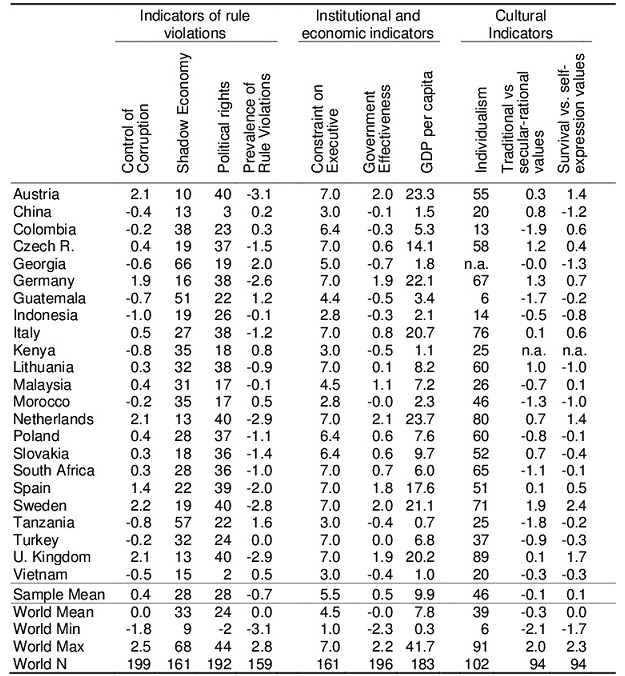
\includegraphics{extended_table1.png}

    \subsection{实验流程}\label{ux5b9eux9a8cux6d41ux7a0b}

    实验设计得很简单但是非常巧妙。实验者被邀请到隔间里坐下,用一个不透明的杯子来摇一个六面的骰子,摇动两次,但是只要求汇报第一次骰子的点数,根据点数的大小参与者可以获得同等大小的报酬,但如果汇报的点数是6,参与者将一无所得。所以我们可以把骰子掷出的点数看作是0,1,2,3,4,5,并得到相应报酬。
  实验规则参与者都会被提前告知,骰子事先经过测试保证正常,摇骰子的结果只有参与者自己知道,最终的物质奖励也是根据各个国家购买力来调整,保证每个单位的奖励相同。因此无论参与者生活在哪个国家,他们面临的鼓励都是相同的,都有动机汇报大的点数(6点看作是最小的点数)。虽然作者无法得知单个参与者是否说谎,但是却能从大样本中得到信息。\\
  从心理学角度看,参与者会在物质诱惑与道德之间做权衡,从而发生一种**
合理说谎** (justified
dishonesty)的现象,反映在本试验中,就是汇报两次掷出的点数中较大的那一个,参与者通过歪曲规则来维持自己诚实的形象,实际上也可以看作一种自我安慰。因此``合理说谎''现象的存在为实验结果提供了一组**
基准值** (benchmarks):点数0汇报的概率为1/36 ≈
2.8\%(只有掷出(6,6)才会汇报点数6);点数1汇报概率为3/36 ≈
8.3\%(掷出(1,1),(6,1),(1,6)三种情况下);点数2、3、4、5的汇报概率应该分别为13.9\%,19.4\%,25\%和30.6\%.

    \subsection{实验结果}\label{ux5b9eux9a8cux7ed3ux679c}

    \subsubsection{总体结果}\label{ux603bux4f53ux7ed3ux679c}

  下图Figure1显示了实验的结果,用** 累计分布函数线** (cumulative
distribution functions, ** CDFs**
)来表示,绿色线表示在PRV较低国家的实验结果,红色线表示在PRV较高国家的实验结果。可以看出,CDFs围绕着基准曲线分布。\\
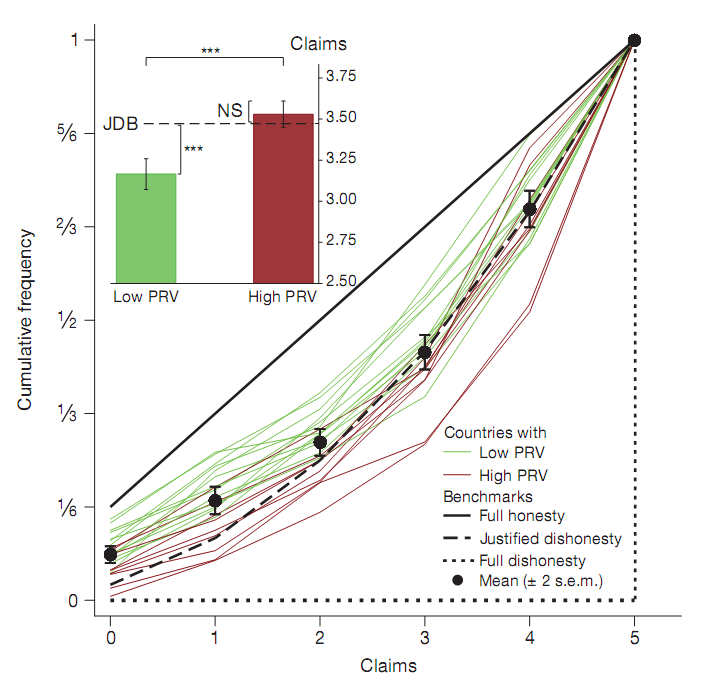
\includegraphics{figure1.png}\\
  结果显示,对``合理说谎''基准值CDF的偏离和国家的PRV是紧密相关的,PRV较低国家的民众诚信品质显著较好。具体Kolmogorov-Smirnov(KS)检验请**
\href{http://files.meetup.com/19659955/CorruptionCorrupts_MainArticle_nature17160.pdf}{阅读原文}**。\\
  就平均汇报点数来看,绝对诚信情况下平均汇报点数为2.5,即平均每人得到2.5个单位的报酬;基准情况下平均汇报点数为3.47。上图中的插图显示,低PRV国家的参与者平均汇报点数为3.17,高PRV国家参与者平均汇报点数为3.53.\\
\#\#\# 分类结果
  上述结果是通过累计分布函数线(CDFs)的方式表示出来的。接着作者通过平均汇报点数、大点数(3,4,5)汇报比例、最高点数5汇报比例、最低点数0汇报比例四种口径,描述了PRV和个人诚信品质之间的关系,如下图Figure2所示,简述如下:\\
  1.PRV和平均汇报点数显著正相关;\\
  2.PRV和大点数汇报比例显著正相关;\\
  3.PRV和最高点数汇报比例没有显著相关;\\
  4.PRV和最低点数汇报比例具有显著相关;\\
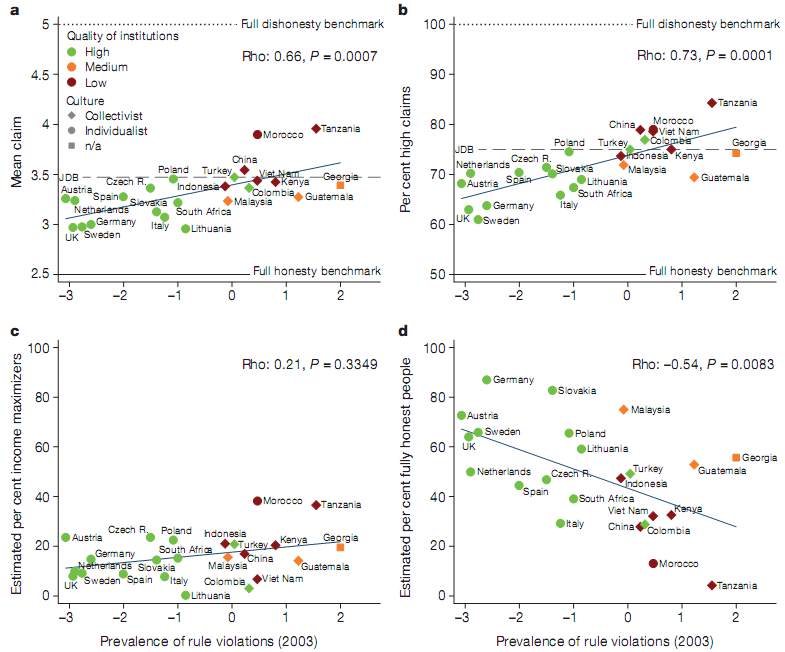
\includegraphics{figure2.png}

    \subsection{回归分析}\label{ux56deux5f52ux5206ux6790}

    作者进一步探究了参与者具体情况如何影响他们的表现,包括参与者对诚信的看法和对他人是否会诚实的看法等,也包括参与者性别、年龄、专业、信仰等社会统计学指标,这些指标同PRV(prevalence
of rule
violations)一道,与汇报点数做回归分析。结果表名只有PRV和参与者对诚信看法这两个解释变量是显著的,像年龄等社会统计学指标都是不显著的。具体回归结果见图Extended
Data Table2.\\
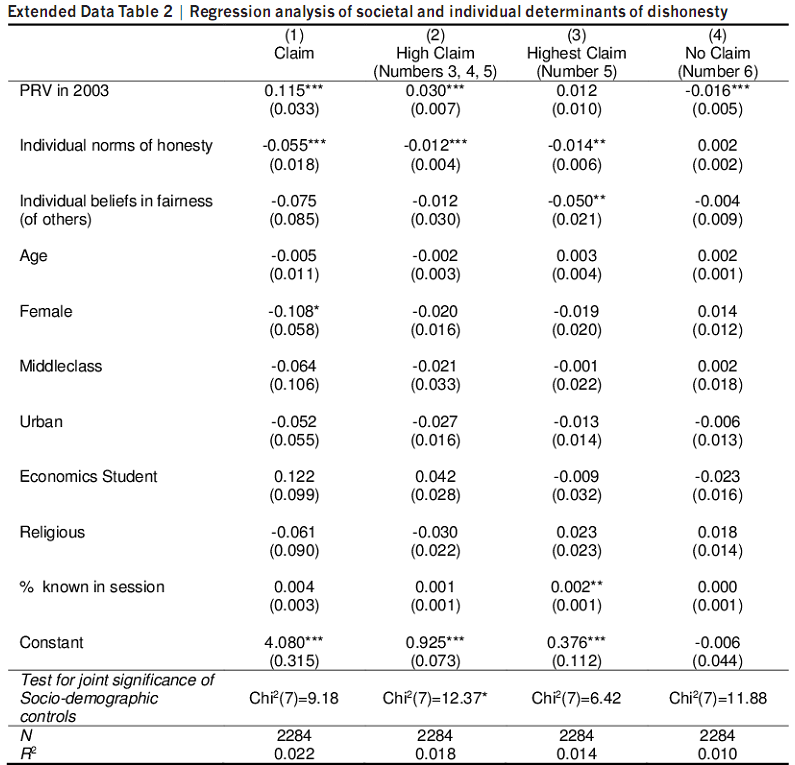
\includegraphics{extended_table2.png}\\
  本文研究主题是制度与文化如何影响个体行为,所以除了使用PRV这个综合性的指标作为解释变量之外,很多具体的制度、文化指标对个人诚信品质影响如何呢?作者使用政府效率、行政集权程度(20世纪末和19世纪末两组)、选举制度公正程度等制度指标,使用个人主义程度、传统价值影响程度、生存还是自我表现程度等文化指标,分别对平均汇报点数(Mean
Claim)做回归,发现这些指标都是和平均汇报点数显著相关的,即都显著影响着个人内在诚信品质。具体回归见图Extended
Data Figure3 和 Extended Data Figure4.\\
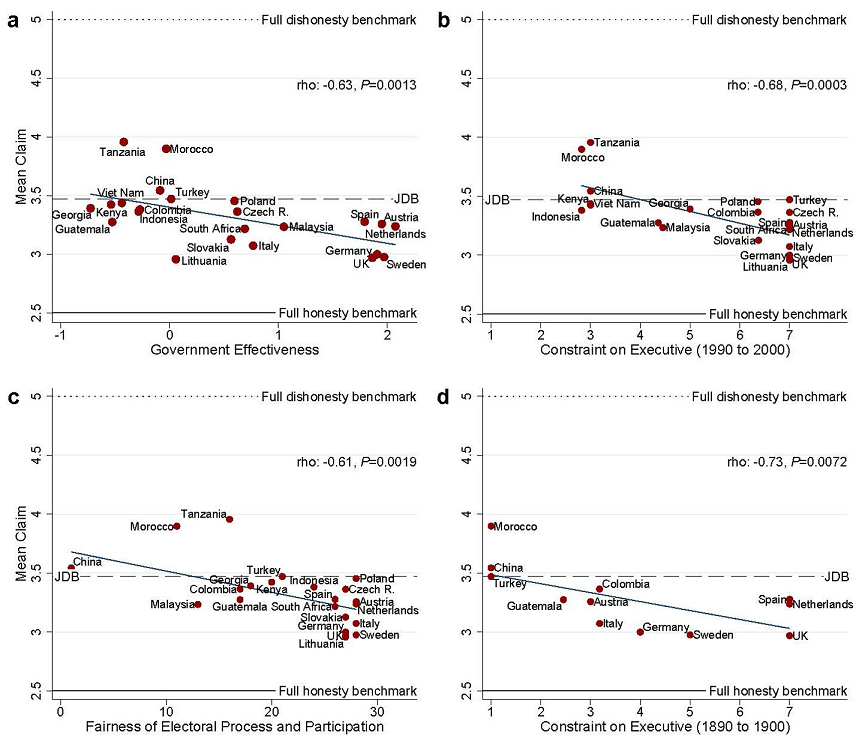
\includegraphics{extended_data_figure3.png}\\
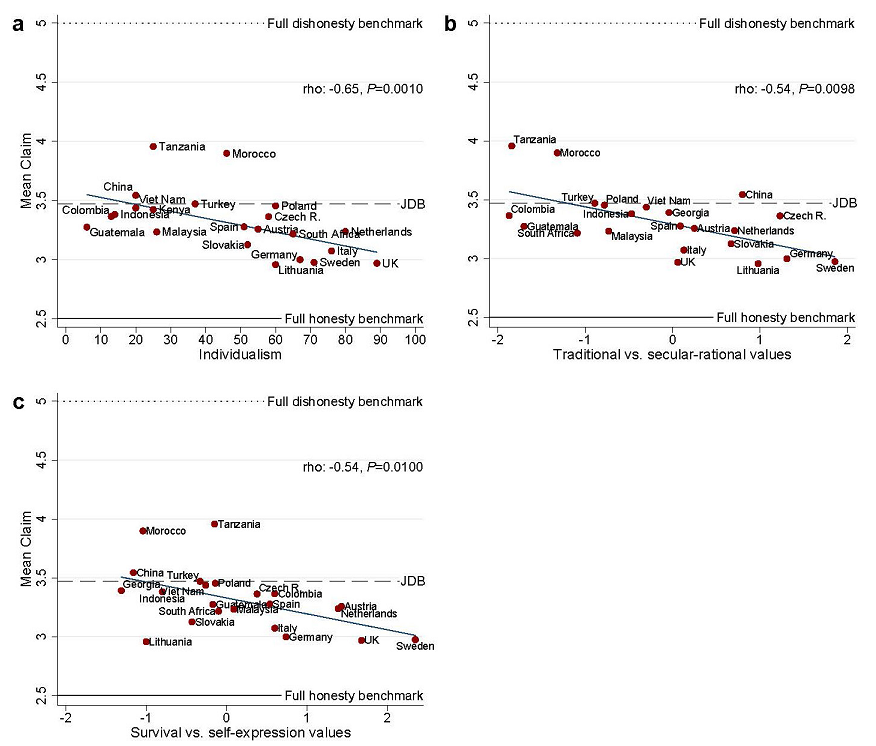
\includegraphics{extended_data_figure4.png}\\
  最后,就以上制度、文化指标是否影响PRV这一问题,作者也做了回归分析,结果是肯定的。以此得出了文章最重要的结论:制度、文化因素通过影响PRV,从而影响了个人内在的诚信品质。具体回归结果请**
阅读原文**

    \subsection{结论}\label{ux7ed3ux8bba}

    综上所述,这篇文章得出的结论是,机构和文化因素影响了PRV(prevalence of
rule
violations),这PRV则通过多种理论可预测的途径(理论分析部分阐述的)影响个人的内在诚信品质,并且人们说谎的模式也与心理学中的``合理说谎''(justified
dishonesty)理论相吻合,说明人们在说谎的同时希望维护自己的诚信形象,于是会扭曲规则进行自我安慰。在具有较低PRV的西方社会,这种自我安慰被最大幅度地限制了,因此公民个人诚信品质更高。确实如**
理论分析**
部分所说的那样,本文通过实验为这些社会学、心理学的理论提供了重要的支持。

    \section{评论}\label{ux8bc4ux8bba}

    \subsection{作者buff}\label{ux4f5cux8005buff}

    这里只介绍第一作者** Simon Gächter**
,1965年出生,奥地利籍经济学家,现在英国诺丁汉大学任教,这里是他的\href{http://www.nottingham.ac.uk/~lezsg1/personalpage.htm}{个人网站}。\\
  Simon
Gächter是行为经济学领域的名人,特别是在经济选择时的心理学研究方面简直是龙头老大,多次在**
Nature** ,** Science** ,** American Economic Review**
发表论文,从网站上长长的论文清单来看,他简直是潮流引流者。因此这篇发表在**
Nature** 上的文章值得一读,只有短短三页,但是每句话都是有价值的。

    \subsection{精巧的思路}\label{ux7cbeux5de7ux7684ux601dux8def}

    本文原文只有短短的三页,实验不仅简单易行,并且能够获得大量有效信息。在实验经济学和行为经济学的研究领域,逻辑严密和设计精巧的实验是至关重要的一环。\\
  首先,要衡量个人内在诚信,需要寻找机构监管能力覆盖不到的领域。在掷骰子的实验中,只有参与者本人知道掷出了多少点,完全符合理想的衡量方式。\\
其次,为了检验** 合理的不诚信** (justified
dishonesty)现象是否存在,实验的规则故意调整为掷两次骰子但是只汇报第一次的点数,而不是只掷一次骰子并且汇报点数,这两种规则有根本的不同。前者为我们提供了一组**
基准值** ,从而在后面的分析中的发挥了巨大作用。\\
  接着,实验规定参与者汇报6点意味着没有报酬是为了什么呢,为什么不能简化规则,规定掷到多少点就有多少奖励?这是那些能够汇报6点的参与者可以看作是完全诚实的人,这是合理而显而易见的。一旦简化规则,汇报1点的人不一定是完全诚实的,因为能够接受1个单位的奖励和完全没有奖励是根本不同的,能够接受空手而归的参与者才是令人信服的完全诚实的人。从而,由于完全诚实的人掷出的点数在0到5之间是等可能的,于是把汇报6点的参与者人数乘以6就可以得到对应实验组里所有完全诚实的人,然后与组中总人数相比,就是一个合理而有意义的衡量个人诚信品质的口径,反映在文章中,就是最后一种衡量口径。所以,实验中衡量汇报点数的四种口径设置也是十分精妙的。\\
  为什么PRV和第三种口径,即最高点数的汇报比例没有显著相关?我想可以解释为,无论在什么社会,人们即使选择说谎和欺瞒也不会油门踩到底,摄取最大利益,而是需要一种类似的**
合理的不诚信** 来自我安慰,故而会寻求次大的利益。\\
  最后,实验的时间安排也很巧妙。PRV(prevalence of rule
violations)来自2003年,而实验2011年至2015年之间进行,保证了参与者们是在2003年的PRV环境中长大,但同时又不会影响PRV,这样就避免了参与者自己解释自己的现象发生。作者使用了OLS这种最基本的回归方法,刻意将精力放在实验上而非拟合上,这与许多带有复杂计量的论文形成对比,使用再大的力气对于隔靴搔痒也是没用的,关键是把皮肤露出来。\\
 我认为文章细节无懈可击,但有一点需要解释清楚:每个国家的参与者都是来自单个城市,比如在中国的237名参与者全部来自上海,那么城市的选择将会影响到参与者的表现,产生结果的不定向偏移,最终对实验结果的影响是:可能影响结论的显著性。

    \subsection{拓展研究}\label{ux62d3ux5c55ux7814ux7a76}

      制度与文化如何影响个体行为?这个话题包含了太多方向和细节。这篇文章博引了很多论文,在此没有列出,请速往**
\href{http://files.meetup.com/19659955/CorruptionCorrupts_MainArticle_nature17160.pdf}{阅读原文}**
。\\
\textgreater{} 本文作者:王耀


    % Add a bibliography block to the postdoc
    
    
    
    \end{document}
